\addcontentsline{toc}{chapter}{Chapitre 5 : Introduction générale} 
\section{Introduction}
Dans ce chapitre, nous analyserons et détaillerons le cinquiéme Sprint . Tout d’abord, on présentons l’organisation de ce Sprint et son Backlog.
Ce que nous avons pu identifier auparavant. Nous présenterons ensuite l'étape d'analyse et fournir des solutions conceptuelles
La relation entre le système et l'utilisateur pour obtenir les résultats souhaités.

\section{Backlog Sprint 5}
Le tableau suivant représante le cinquiéme sprint avec les différents User Story.

\begin{table*}[h]
    \begin{center} 
    \begin{tabular}{|p{3cm}|p{6cm}|p{3cm}|p{1.9cm}|p{2cm}|} \hline 
          Module &  User Stories &  Tache &  Complexité & Estimation \\ \hline
          Gestion des avis & En tant que visiteur je veux consulter les avis &Dévelopement du front end & \centering L &  1 jour  \\  \hline
          & En tant que étudiant je veux consulter les avis & Dévelelopement back end & \centering H & 4 jous \\ \hline
          & En tant que étudiant je veux donner un avis & Dévelelopement back end & \centering H & 4 jous \\ \hline
          & En tant que professeur je veux consulter les avis & Developement back end &  \centering M & 2 jours \\ \hline
          & En tant que professeur je veux donner un avis & Developement back end &  \centering M & 2 jours \\ \hline  
          & En tant que professeur je veux donner un avis & Developement back end &  \centering M & 2 jours \\ \hline  
          & En tant que admin je veux consulter les avis & Developement back end &  \centering M & 2 jours \\ \hline  
          & En tant que admin je veux supprimer un avis & Developement back end &  \centering M & 2 jours \\ \hline  
            
    \end{tabular}
  \end{center}
  \caption{ Backlog sprint1}
\label{tab:bert_res}
\end{table*}



\section{analyse fonctionnelle}
Dans cette partie on va présenter les besoins fonctionnels du sprint"Gestion des avis"  qui ce déroule entre quelques acteurs : 
\begin{itemize}
    \item visiteur 
    \item administrateur 
    \item étudiant
    \item professeur 
\end{itemize}
\section{Diagramme de cas d'utilisation détaillé }

\begin{figure}[h]
    \centering
    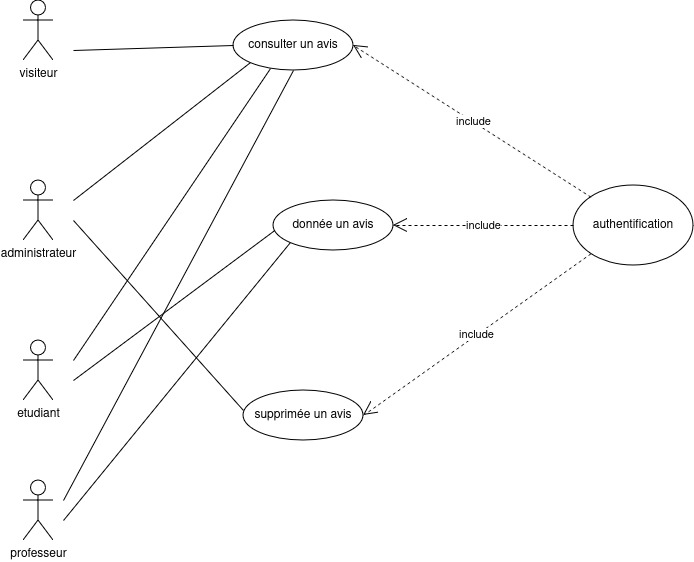
\includegraphics[width=0.7\linewidth]{pages/image/asma-usecase-gestion_des_avis.jpg}
    \caption{ diagramme de cas d'utilisation pour la gestion d'avis}
    \label{fig:enter-label}
\end{figure}
\newpage
\section{Déscription textuelle }

\begin{table*}[h]
    \begin{center} 
    \begin{tabular}{|p{4cm}|p{9cm}|}  \hline 
       Cas d'utilisation& Gestion des avis \\ \hline
       Acteur& Etudiant,Administrateur , visiteur ,professeur\\ \hline
       Précondition&  L'étudiants,l'administrateur ou le professeur doive être authentifiés au plateforme &  \\ \hline
       Post condition& Un avis sera ajouté à la liste des avis.\\ \hline


       
       Scénario nominale& Le systéme affiche la liste des exercies  \\
                        & L'étudiant sélectionne un exercies à le faire \\
                        & L'étudiant termine a faire et va donner un avis sur l'exercies \\
                        & L'admin peut supprimer un avis \\ \hline
          
                       
       Scénario alternatif& Le système renvoie un message d’erreur et signale à l’étudiant de
recommencer en cas d’erreur de synchronisation. \\  \hline
  \end{tabular}
  \end{center}
  \caption{ Déroulement de cas d'utilisation}
\label{tab:bert_res}
\end{table*}

\section{Conception }

La figure  décrit le déroulement du cas d’utilisation « donner un avis » pour le visteur.
\begin{figure}[h!]
    \centering
    \includegraphics[width=0.8\linewidth]{}
    \caption{Diagramme de séquance «Gestion des avis - visiteur»}
    \label{fig:enter-label}
\end{figure}
\\ 

Le diagramme ci-dessous représente le diagramme de séquence du cas d’utilisation « Gestion des avis » pour l'etudiant 
\begin{figure}[h!]
    \centering
    \includegraphics[width=0.8\linewidth]{}
    \caption{Diagramme de séquance «donner un avis - etudiant »}
    \label{fig:enter-label}
\end{figure}
\\


Le diagramme ci-dessous représente le diagramme de séquence du cas d’utilisation « Gestion des avis » pour le professeur 
\begin{figure}[h!]
    \centering
    \includegraphics[width=0.8\linewidth]{}
    \caption{Diagramme de séquance «donner un avis - professeur»}
    \label{fig:enter-label}
\end{figure}
\\


Le diagramme ci-dessous représente le diagramme de séquence du cas d’utilisation « Gestion des avis » pour l'administrateur 
\begin{figure}[h!]
    \centering
    \includegraphics[width=0.8\linewidth]{}
    \caption{Diagramme de séquance «donner un avis - administrateur »}
    \label{fig:enter-label}
\end{figure}
\\


\section{Diagramme de classe condidate}
La figure  représente les différentes classes candidates du ce Sprint.
\begin{figure}[h!]
    \centering
    \includegraphics[width=0.5\linewidth]{}
    \caption{Diagramme de classe "ajouter un avis"}
    \label{fig:enter-label}
\end{figure}

\section{Réalisation}
cette figure représante l'interface des avis données sur les supports de cours pour un visiteur qui n'est pas inscrit au plateforme:

\begin{figure}[h!]
    \centering
    \includegraphics[width=0.5\linewidth]{}
    \caption{Interface utlisateur pour consulter les avis existante}
    \label{fig:enter-label}
\end{figure}
\\

Cette figure représante l'interface des avis données sur les supports de cours pour un étudiant:
\begin{figure}[h!]
    \centering
    \includegraphics[width=0.5\linewidth]{}
    \caption{Interface utilisateur pour un étudiant qui a ajouté un avis}
    \label{fig:enter-label}
\end{figure}


\section{Conclusion:}
En conclusion ,dans cette chapitre nous avons exploré les élements clés de la procedure de la gestion des avis pour notre plateforme